\documentclass[12pt]{article}
\usepackage{latexblog}

% ============================================================
% Blog Metadata
% ============================================================
\blogtitle{Knative简介}
\blogdate{2023-01-10}
\blogtags{云计算, 容器化}
\bloglang{zh}
\blogsummary{}

\begin{document}
\makeblogtitle

Knative是一个开源的Serverless平台，它实现了一套架构无关的Serverless系统。本文介绍其安装及入门使用。

\section{安装Knative}\label{ux5b89ux88c5knative}

\subsection{Option 1：使用Docker Desktop + minikube + quickstart}\label{option-1ux4f7fux7528docker-desktop-minikube-quickstart}

体验Knative时，首先需要在本机进行安装。基于以下的环境进行安装：

\begin{itemize}
\tightlist
\item
  Windows 11
\item
  Docker Desktop
\item
  minikube
\end{itemize}

之所以这样选择，是因为首先Docker Desktop最为流行，minikube（以及kind）是Knative/Tekton官方例子中推荐的选择，因此肯定是兼容的。之前更多时候我青睐于k3s，因为k3s是真正的production-ready的轻量级k8s版本，但是因为Knative有单独的网络层，在k3s上安装时需要特别处理一下，考虑到复杂性还是用minikube吧。minikube必须要Docker或者其他的运行时支持。

\begin{Shaded}
\begin{Highlighting}[]
\CommentTok{\# 先启动docker desktop}
\ExtensionTok{minikube}\NormalTok{ start}
\end{Highlighting}
\end{Shaded}

minikube启动时会下载一些镜像，因此如果没有翻墙很可能下载不了。另外有时候会出现卡死的情况， 解决方式是，删掉重新来过：

\begin{Shaded}
\begin{Highlighting}[]
\ExtensionTok{minikube}\NormalTok{ delete}
\FunctionTok{rm} \AttributeTok{{-}rf}\NormalTok{ \textasciitilde{}/.minkube}
\ExtensionTok{minikube}\NormalTok{ start}
\end{Highlighting}
\end{Shaded}

\subsubsection{使用quickstart插件安装Knative}\label{ux4f7fux7528quickstartux63d2ux4ef6ux5b89ux88c5knative}

Knative支持一种叫quickstart的插件安装机制，可以比较方便的开启一个本地环境。完整的安装过程可以参考\href{https://knative.dev/docs/getting-started/quickstart-install/}{官方文档}，仅列出安装的文件：

\begin{itemize}
\tightlist
\item
  kn.exe
\item
  kn-func.exe
\item
  kn-quickstart.exe
\end{itemize}

这些都需要加入到系统Path之中。然后运行安装：

\begin{Shaded}
\begin{Highlighting}[]
\ExtensionTok{kn}\NormalTok{ quickstart minikube}
\end{Highlighting}
\end{Shaded}

这一步后还需要执行一个命令，并保证其始终运行（可以单独开一个Terminal窗口执行）：

\begin{Shaded}
\begin{Highlighting}[]
\ExtensionTok{minikube}\NormalTok{ tunnel }\AttributeTok{{-}{-}profile}\NormalTok{ knative}
\end{Highlighting}
\end{Shaded}

安装成功后，应该可以能够列出Knative profile:

\begin{Shaded}
\begin{Highlighting}[]
\ExtensionTok{minikube}\NormalTok{ profile list}
\end{Highlighting}
\end{Shaded}

\pandocbounded{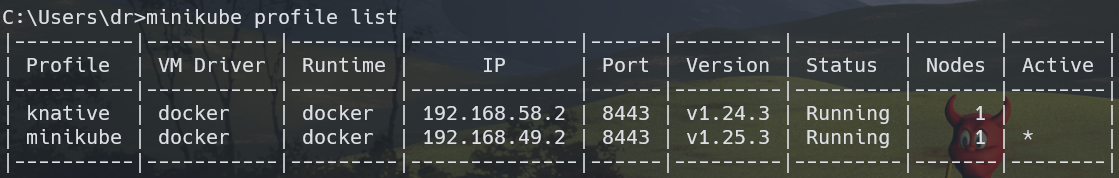
\includegraphics[keepaspectratio]{images/Knative-profile.png}}

\subsection{Option 2：使用WSL2 + Docker（Linux） + minikube安装（推荐）}\label{option-2ux4f7fux7528wsl2-dockerlinux-minikubeux5b89ux88c5ux63a8ux8350}

使用Docker Desktop有一个不好的地方是，容器不能直接在宿主机上访问， 因此直接在Linux中部署Docker和Minikube是不能直接访问到k8s的host上的。 所以直接在WSL中安装docker和minikube，这样可以更容易使用。

\subsubsection{安装Docker}\label{ux5b89ux88c5docker}

\begin{Shaded}
\begin{Highlighting}[]
\FunctionTok{sudo}\NormalTok{ apt{-}get update}
\FunctionTok{sudo}\NormalTok{ apt{-}get install }\DataTypeTok{\textbackslash{}}
\NormalTok{    ca{-}certificates }\DataTypeTok{\textbackslash{}}
\NormalTok{    curl }\DataTypeTok{\textbackslash{}}
\NormalTok{    gnupg }\DataTypeTok{\textbackslash{}}
\NormalTok{    lsb{-}release}

\FunctionTok{sudo}\NormalTok{ mkdir }\AttributeTok{{-}m}\NormalTok{ 0755 }\AttributeTok{{-}p}\NormalTok{ /etc/apt/keyrings}
\ExtensionTok{curl} \AttributeTok{{-}fsSL}\NormalTok{ https://download.docker.com/linux/ubuntu/gpg }\KeywordTok{|} \FunctionTok{sudo}\NormalTok{ gpg }\AttributeTok{{-}{-}dearmor} \AttributeTok{{-}o}\NormalTok{ /etc/apt/keyrings/docker.gpg}

\BuiltInTok{echo} \DataTypeTok{\textbackslash{}}
  \StringTok{"deb [arch=}\VariableTok{$(}\ExtensionTok{dpkg} \AttributeTok{{-}{-}print{-}architecture}\VariableTok{)}\StringTok{ signed{-}by=/etc/apt/keyrings/docker.gpg] https://download.docker.com/linux/ubuntu }\DataTypeTok{\textbackslash{}}
\StringTok{  }\VariableTok{$(}\ExtensionTok{lsb\_release} \AttributeTok{{-}cs}\VariableTok{)}\StringTok{ stable"} \KeywordTok{|} \FunctionTok{sudo}\NormalTok{ tee /etc/apt/sources.list.d/docker.list }\OperatorTok{\textgreater{}}\NormalTok{ /dev/null}

\FunctionTok{sudo}\NormalTok{ apt{-}get update}

\FunctionTok{sudo}\NormalTok{ apt{-}get install docker{-}ce docker{-}ce{-}cli containerd.io docker{-}buildx{-}plugin docker{-}compose{-}plugin}

\FunctionTok{sudo}\NormalTok{ service docker start}
\end{Highlighting}
\end{Shaded}

注意WSL2默认不支持Systemd，因此只能使用service xx start/stop方式启动和停止。

\subsubsection{安装Kubectl}\label{ux5b89ux88c5kubectl}

\begin{Shaded}
\begin{Highlighting}[]
\FunctionTok{sudo}\NormalTok{ apt{-}get install }\AttributeTok{{-}y}\NormalTok{ apt{-}transport{-}https}
\FunctionTok{sudo}\NormalTok{ curl }\AttributeTok{{-}fsSLo}\NormalTok{ /etc/apt/keyrings/kubernetes{-}archive{-}keyring.gpg https://packages.cloud.google.com/apt/doc/apt{-}key.gpg}
\BuiltInTok{echo} \StringTok{"deb [signed{-}by=/etc/apt/keyrings/kubernetes{-}archive{-}keyring.gpg] https://apt.kubernetes.io/ kubernetes{-}xenial main"} \KeywordTok{|} \FunctionTok{sudo}\NormalTok{ tee /etc/apt/sources.list.d/kubernetes.list}

\FunctionTok{sudo}\NormalTok{ apt{-}get update}
\FunctionTok{sudo}\NormalTok{ apt{-}get install }\AttributeTok{{-}y}\NormalTok{ kubectl}
\end{Highlighting}
\end{Shaded}

\subsubsection{安装Minikube}\label{ux5b89ux88c5minikube}

选择Minikube作为本地Kubernetes开发有以下优点：

\begin{itemize}
\tightlist
\item
  跨平台支持（Windows/Mac/Linux）
\item
  默认支持K8s的基本特性，如Service、Ingress、PV、LB等
\item
  支持创建多个集群
\item
  支持Nvidia GPU，对机器学习友好
\end{itemize}

\begin{Shaded}
\begin{Highlighting}[]
\ExtensionTok{curl} \AttributeTok{{-}LO}\NormalTok{ https://storage.googleapis.com/minikube/releases/latest/minikube\_latest\_amd64.deb}
\FunctionTok{sudo}\NormalTok{ dpkg }\AttributeTok{{-}i}\NormalTok{ minikube\_latest\_amd64.deb}
\end{Highlighting}
\end{Shaded}

注意：Minikube依赖Docker 服务，必须启动起来。

\subsubsection{创建K8s集群}\label{ux521bux5efak8sux96c6ux7fa4}

\begin{Shaded}
\begin{Highlighting}[]
\ExtensionTok{minikube}\NormalTok{ start }\AttributeTok{{-}p}\NormalTok{ kfaas{-}cluster }\DataTypeTok{\textbackslash{}}
    \AttributeTok{{-}{-}memory}\OperatorTok{=}\NormalTok{8192 }\DataTypeTok{\textbackslash{}}
    \AttributeTok{{-}{-}cpus}\OperatorTok{=}\NormalTok{6 }\DataTypeTok{\textbackslash{}}
    \AttributeTok{{-}{-}driver}\OperatorTok{=}\NormalTok{docker }\DataTypeTok{\textbackslash{}}
    \AttributeTok{{-}{-}kubernetes{-}version}\OperatorTok{=}\NormalTok{v1.25.6 }\DataTypeTok{\textbackslash{}}
    \AttributeTok{{-}{-}disk{-}size}\OperatorTok{=}\NormalTok{50g }\DataTypeTok{\textbackslash{}}
    \AttributeTok{{-}{-}insecure{-}registry}\OperatorTok{=}\StringTok{\textquotesingle{}10.0.0.0/24\textquotesingle{}}
\end{Highlighting}
\end{Shaded}

\subsubsection{启用Registry插件}\label{ux542fux7528registryux63d2ux4ef6}

\begin{Shaded}
\begin{Highlighting}[]
\ExtensionTok{minikube} \AttributeTok{{-}p}\NormalTok{ kfaas{-}cluster addons enable registry}
\end{Highlighting}
\end{Shaded}

\subsubsection{创建和配置默认的Namespace}\label{ux521bux5efaux548cux914dux7f6eux9ed8ux8ba4ux7684namespace}

至此，Kubernetes部署完成，可以创建一个Namespace用来进行开发测试用，并配置为默认的命名空间，例如：

\begin{Shaded}
\begin{Highlighting}[]
\ExtensionTok{kubectl}\NormalTok{ create namespace develop}
\ExtensionTok{kubectl}\NormalTok{ config set{-}context }\AttributeTok{{-}{-}current} \AttributeTok{{-}{-}namespace}\OperatorTok{=}\NormalTok{develop}
\end{Highlighting}
\end{Shaded}

\subsubsection{安装Knative}\label{ux5b89ux88c5knative-1}

CRD定义是安装Knative Serving或者Knative Eventing的依赖项，因此需要先安装。

\begin{Shaded}
\begin{Highlighting}[]
\ExtensionTok{kubectl}\NormalTok{ apply }\DataTypeTok{\textbackslash{}}
  \AttributeTok{{-}{-}filename}\NormalTok{ https://github.com/knative/serving/releases/download/knative{-}v1.9.0/serving{-}crds.yaml }\DataTypeTok{\textbackslash{}}
  \AttributeTok{{-}{-}filename}\NormalTok{ https://github.com/knative/eventing/releases/download/knative{-}v1.9.0/eventing{-}crds.yaml}
\end{Highlighting}
\end{Shaded}

完成后，可以查看已经安装的API版本，例如：

\begin{Shaded}
\begin{Highlighting}[]
\ExtensionTok{kubectl}\NormalTok{ api{-}resources }\AttributeTok{{-}{-}api{-}group}\OperatorTok{=}\StringTok{\textquotesingle{}serving.knative.dev\textquotesingle{}}
\end{Highlighting}
\end{Shaded}

其中，Knative主要有以下一些API组：

\begin{itemize}
\tightlist
\item
  serving.knative.dev
\item
  messaging.knative.dev
\item
  eventing.knative.dev
\item
  sources.knative.dev
\end{itemize}

安装Knative Serving

\begin{Shaded}
\begin{Highlighting}[]
\ExtensionTok{kubectl}\NormalTok{ apply }\AttributeTok{{-}f}\NormalTok{ https://github.com/knative/serving/releases/download/knative{-}v1.9.0/serving{-}core.yaml}
\ExtensionTok{kubectl}\NormalTok{ apply }\AttributeTok{{-}f}\NormalTok{ https://github.com/knative/eventing/releases/download/knative{-}v1.9.0/eventing{-}core.yaml}
\ExtensionTok{kubectl}\NormalTok{ apply }\AttributeTok{{-}f}\NormalTok{ https://github.com/knative/eventing/releases/download/knative{-}v1.9.0/in{-}memory{-}channel.yaml}
\ExtensionTok{kubectl}\NormalTok{ apply }\AttributeTok{{-}f}\NormalTok{ https://github.com/knative/eventing/releases/download/knative{-}v1.9.0/mt{-}channel{-}broker.yaml}
\end{Highlighting}
\end{Shaded}

安装后，需耐心等待各个资源创建成功。

\begin{Shaded}
\begin{Highlighting}[]
\ExtensionTok{kubectl}\NormalTok{ get pods }\AttributeTok{{-}n}\NormalTok{ knative{-}serving}
\ExtensionTok{kubectl}\NormalTok{ get pods }\AttributeTok{{-}n}\NormalTok{ knative{-}eventing}
\end{Highlighting}
\end{Shaded}

Knative官方提供了Kourier的Ingress实现（目前已经GA）。

\begin{Shaded}
\begin{Highlighting}[]
\ExtensionTok{kubectl}\NormalTok{ apply }\AttributeTok{{-}f}\NormalTok{ https://github.com/knative{-}sandbox/net{-}kourier/releases/download/knative{-}v1.9.0/kourier.yaml}
\ExtensionTok{kubectl}\NormalTok{ patch configmap/config{-}network }\DataTypeTok{\textbackslash{}}
  \AttributeTok{{-}n}\NormalTok{ knative{-}serving }\DataTypeTok{\textbackslash{}}
  \AttributeTok{{-}{-}type}\NormalTok{ merge }\DataTypeTok{\textbackslash{}}
  \AttributeTok{{-}p} \StringTok{\textquotesingle{}\{"data":\{"ingress.class":"kourier.ingress.networking.knative.dev"\}\}\textquotesingle{}}
\VariableTok{ksvc\_domain}\OperatorTok{=}\StringTok{"}\DataTypeTok{\textbackslash{}"}\StringTok{data}\DataTypeTok{\textbackslash{}"}\StringTok{:\{}\DataTypeTok{\textbackslash{}"}\StringTok{"}\VariableTok{$(}\ExtensionTok{minikube} \AttributeTok{{-}p}\NormalTok{ kfaas{-}cluster ip}\VariableTok{)}\StringTok{".nip.io}\DataTypeTok{\textbackslash{}"}\StringTok{: }\DataTypeTok{\textbackslash{}"\textbackslash{}"}\StringTok{\}"}
\ExtensionTok{kubectl}\NormalTok{ patch configmap/config{-}domain }\DataTypeTok{\textbackslash{}}
    \AttributeTok{{-}n}\NormalTok{ knative{-}serving }\DataTypeTok{\textbackslash{}}
    \AttributeTok{{-}{-}type}\NormalTok{ merge }\DataTypeTok{\textbackslash{}}
    \AttributeTok{{-}p} \StringTok{"\{}\VariableTok{$ksvc\_domain}\StringTok{\}"}
\end{Highlighting}
\end{Shaded}

\subsubsection{安装Knative CLI}\label{ux5b89ux88c5knative-cli}

\begin{Shaded}
\begin{Highlighting}[]
\FunctionTok{wget}\NormalTok{ https://github.com/knative/client/releases/download/knative{-}v1.9.0/kn{-}linux{-}amd64}
\FunctionTok{sudo}\NormalTok{ mv kn{-}linux{-}amd64 /usr/local/bin/kn}
\FunctionTok{sudo}\NormalTok{ chmod +x /usr/local/bin/kn}
\end{Highlighting}
\end{Shaded}

\section{Hello World!}\label{hello-world}

\subsection{Knative Functions}\label{knative-functions}

通过func命令（或者kn func）来创建一个Function，这里以Python为例：

\begin{Shaded}
\begin{Highlighting}[]
\ExtensionTok{kn}\NormalTok{ func create }\AttributeTok{{-}l}\NormalTok{ python helloworld}

\BuiltInTok{cd}\NormalTok{ helloworld}
\ExtensionTok{kn}\NormalTok{ func run}
\end{Highlighting}
\end{Shaded}

这里运行时会提示提供一个registry名称，暂时可以随便输入一个即可。第一次运行需要进行构建， 这个构建过程稍微会需要一点时间。运行后，会启动8080端口，可以在浏览器访问：

\pandocbounded{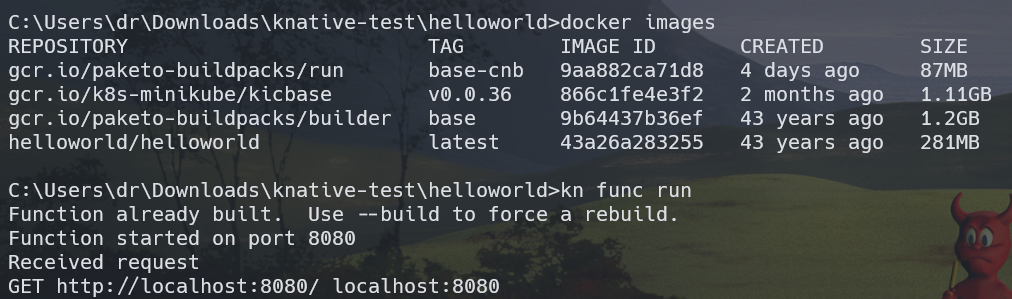
\includegraphics[keepaspectratio]{images/Knative-func-helloworld.png}}

\subsection{Hello world（WSL+Minikube方式部署）}\label{hello-worldwslminikubeux65b9ux5f0fux90e8ux7f72}

\begin{Shaded}
\begin{Highlighting}[]
\ExtensionTok{kn}\NormalTok{ service create helloworld{-}go }\AttributeTok{{-}{-}image}\NormalTok{ gcr.io/knative{-}samples/helloworld{-}go}
\end{Highlighting}
\end{Shaded}

访问：注意这里不能直接通过URL访问，需要使用Kurior的SVC并设置Header。

\begin{Shaded}
\begin{Highlighting}[]
\ExtensionTok{curl} \AttributeTok{{-}H} \StringTok{"Host: helloworld{-}go.develop.192.168.49.2.nip.io"}\NormalTok{ http://192.168.49.2:32117}
\end{Highlighting}
\end{Shaded}

参考：

\begin{itemize}
\tightlist
\item
  https://www.archcloudlabs.com/projects/diving-into-kubernetes/
\item
  https://www.reddit.com/r/kubernetes/comments/v1a6ay/running\_kubernetes\_locally\_and\_minikube\_vs/
\item
  https://docs.google.com/spreadsheets/d/1ZT8m4gpvh6xhHYIi4Ui19uHcMpymwFXpTAvd3EcgSm4/edit\#gid=0
\item
  https://knative.dev/docs/getting-started/quickstart-install/
\item
  https://docs.docker.com/engine/install/ubuntu/\#install-from-a-package
\item
  https://redhat-developer-demos.github.io/knative-tutorial/knative-tutorial/index.html
\item
  https://kubernetes.io/docs/tasks/tools/install-kubectl-linux/
\item
  https://github.com/knative/serving/issues/11624
\item
  https://github.com/knative-sandbox/net-kourier/issues/992
\item
  https://knative.dev/docs/install/yaml-install/serving/install-serving-with-yaml/\#install-a-networking-layer
\end{itemize}


\end{document}
